% === Week 1 ===
\chapter*{Week 1: grondslagen statistiek en datavisualisatie}

\section*{Hoofdstuk 1}

\question{1.m1}{Bij een verkeersonderzoek is een van de grootheden die wordt genoteerd het merk van de passerende auto's. Dit merk is ...}
\begin{enumerate}[label=(\alph*)]
    \item een ratiovariabele
    \item een kwantitatieve variabele
    \item een nominale variabele.
    \item geen variabele
\end{enumerate}
\answer{Het juiste antwoord is (c)}

\question{1.m2}{Zie tabel. Bij de mannen is het percentage dat het eens is met de voorgestelde maatregelen gelijk aan ...}
\begin{enumerate}[label=(\alph*)]
    \item $41,7\%$
    \item $10\%$
    \item $25\%$
    \item $22,7\%$
\end{enumerate}
\answer{Het juiste antwoord is (d)}

\question{1.m3}{Zie tabel. De groep mensen die het oneens is met de maatregelen bestaat voor ... uit vrouwen.}
\begin{enumerate}[label=(\alph*)]
    \item $20\%$
    \item $56\%$
    \item $50\%$
    \item $40\%$
\end{enumerate}
\answer{Het juiste antwoord is (c)}

Bij de reisorganisatie $P$-tours heeft men bijgehouden hoeveel geboekte passagiers kort voor het vertrek van een busreis hun reis afzeggen.
Voor 80 busreizen leverde dit de volgende tabel:

\begin{table}[h!]
    \centering
    \caption*{Aantal passagiers per busreis dat annuleert}
    \begin{tabular}{ccc}
        \toprule
            {\bfseries Nummer} & {\bfseries Aantal afzeggers} & {\bfseries Frequentie} \\
        \midrule
            1 & 0 -< 5 & 36 \\
            2 & 5 -< 8 & 24 \\
            3 & 8 -< 12 & 8 \\
            4 & 12 -< 16 & 6 \\
            5 & 16 -< 20 & 4 \\
            6 & 20 en hoger & 2 \\
        \midrule    
            Totaal & & $80$ \\
        \bottomrule
    \end{tabular}
\end{table}

\question{1.m4}{De klassenbreedte bij 0 -< 5 bedraagt \dots}
\begin{enumerate}[label=(\alph*)]
    \item $5$
    \item $4$
    \item $4,5$
    \item $36$
\end{enumerate}
\answer{Het juiste antwoord is (a)}

\question{1.m5}{De relatieve frequentie van de klasse 16 -< 20 bedraagt \dots}
\begin{enumerate}[label=(\alph*)]
    \item $0,05$
    \item $4$
    \item $16$
    \item $0,20$
\end{enumerate}
\answer{Het juiste antwoord is (a)}

\question{1.m6}{Het klassenmidden van de klasse 8 -< 12 bedraagt \dots}
\begin{enumerate}[label=(\alph*)]
    \item $2$
    \item $10$
    \item $10,5$
    \item $9,5$
\end{enumerate}
\answer{Het juiste antwoord is (d)}

\question{1.3}{Geef voor elk van de volgende gevallen aan of de genoemde verzameling} als een steekproef of als een populatie mag worden beschouwd:
\begin{enumerate}[label=(\alph*)]
    \item de commissarissen van de koning van de 12 Nederlandse provincies
    \item de 200 personen die zijn ge\"interviewd bij een straatenqu\^ete
    \item de 150 automobilisten die moesten stoppen voor een alcoholcontrole
    \item de 740 leden van een studentenvereniging
    \item de 38 klanten die tussen 11.00 en 12.00 uur een postkantoor binnenkomen
    \item de 12000 verzekerden bij een verzekeringsmaatschappij
    \item de 20 nummers die worden gedraaid in een muziekprogramma op de radio
\end{enumerate}

\answer{
    \begin{enumerate}[label=(\alph*)]
        \item Populatie
        \item Steekproef
        \item Steekproef
        \item Populatie
        \item Steekproef
        \item Populatie
        \item Steekproef
    \end{enumerate} 
}

\question{1.4}{Geef voor de volgende variabelen aan of deze een nominale, ordinale, interval- of ratioschaal heeft:

    \begin{enumerate}[label=(\alph*)]
        \item de speelduur van een dvd
        \item de kleur van tulpen
        \item de industrietak waarin werknemers een baan hebben
        \item de jaaromzet (in euro) van bedrijven
        \item het aantal sterren dat de moeilijkheidsgraad van puzzelboekjes aangeeft
        \item de hoogte boven de zeespiegel van wintersportdorpen
    \end{enumerate}
}

\answer{
    \begin{enumerate}[label=(\alph*)]
        \item Ratio
        \item Nominaal
        \item Nominaal
        \item Ratio
        \item Ordinaal
        \item Ratio
    \end{enumerate} 
}

\question{1.7}{Een groep van dertig eerstejaarsstudenten is een aantal vragen voorgelegd. Dit betrof:
    \begin{itemize}
        \item Leeftijd
        \item Woonsituatie (z=zelfstandig, o=bij ouders)
        \item Geslacht (m=man, v=vrouw)
        \item De maandelijke bestedingen aan voedsel en drank
        \item De score voor het tentamen statistiek
    \end{itemize}
    In het boek staan de resultaten in een tabel.
}

\begin{enumerate}[label=(\alph*)]
    \item Geef aan op welk type schaal de vijf variabelen worden gemeten
    \answer{Naam: nominaal, leeftijd: ratio, woonsituatie: nominaal, geslacht: nominaal, besteding: ratio, score: interval}

    \item Maak een frequentieverdeling van de leeftijden
    \answer{
        \begin{center}
            \begin{tabular}{cc}
                \toprule
                    {\bfseries Leeftijd} & {\bfseries Frequentie} \\
                \midrule
                    $18$ & $2$ \\
                    $19$ & $5$ \\
                    $20$ & $6$ \\
                    $21$ & $6$ \\
                    $22$ & $5$ \\
                    $23$ & $3$ \\
                    $24$ & $1$ \\
                    $25$ & $1$ \\
                    $26$ & $1$ \\
                \midrule    
                    Totaal & $30$ \\
                \bottomrule
            \end{tabular}
        \end{center}
    }
    \item Teken een histogram van de bestedingen. Begin met ondergrens \euro 250.
    \answer{
        \begin{center}
            \resizebox{0.9\textwidth}{!}{
                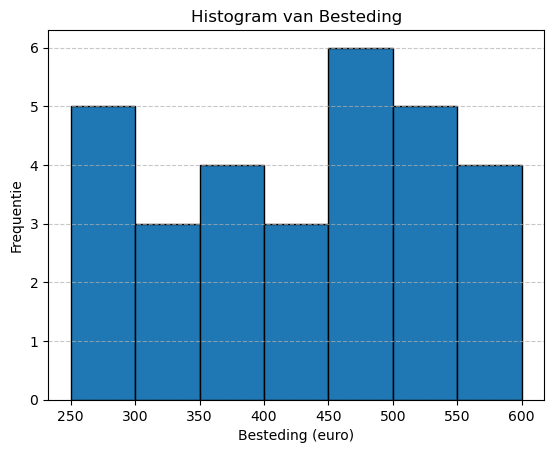
\includegraphics{opg1.7c.png}
            }
        \end{center}
    }
    \item Maak een klassenindeling van de scores voor mannen en vrouwen afzonderlijk. 
    Kies voor de klassen 10 eenheden en verwerk de resultaten in een kruistabel. 
    Bereken ook de procentuele frequenties van de scoreklassen voor de mannen en vrouwen afzonderlijk.
    \answer{
        De absolute frequentieverdeling van de scoreklassen naar geslacht is gelijk aan

        \begin{center}
            \begin{tabular}{ccc|c}
                \toprule
                    {\bfseries Scoreklasse} & {\bfseries Man} & {\bfseries Vrouw} & {\bfseries Totaal} \\
                \midrule
                    $[30, 40)$ & $1$ & $0$ & $1$ \\
                    $[40, 50)$ & $1$ & $5$ & $6$ \\
                    $[50, 60)$ & $3$ & $0$ & $3$ \\
                    $[60, 70)$ & $4$ & $2$ & $6$ \\
                    $[70, 80)$ & $2$ & $4$ & $6$ \\
                    $[80, 90)$ & $4$ & $1$ & $5$ \\
                    $[90, 100)$ & $3$ & $0$ & $3$ \\
                \midrule    
                    Totaal & $18$ & $12$ & $30$ \\
                \bottomrule
            \end{tabular}
        \end{center}
        De relatieve frequentieverdeling van de scoreklassen naar geslacht is gelijk aan

        \begin{center}
            \begin{tabular}{ccc|c}
                \toprule
                    {\bfseries Scoreklasse} & {\bfseries Man} & {\bfseries Vrouw} & {\bfseries Totaal} \\
                \midrule
                    $[30, 40)$ & $5.6$ & $0.0$ & $5.6$ \\
                    $[40, 50)$ & $5.6$ & $41.7$ & $47.3$ \\
                    $[50, 60)$ & $16.7$ & $0.0$ & $16.7$ \\
                    $[60, 70)$ & $22.2$ & $16.7$ & $38.9$ \\
                    $[70, 80)$ & $11.1$ & $33.3$ & $44.4$ \\
                    $[80, 90)$ & $22.2$ & $8.3$ & $30.5$ \\
                    $[90, 100)$ & $16.7$ & $0.0$ & $16.7$ \\
                \midrule    
                    Totaal & $60$ & $40$ & $100$ \\
                \bottomrule
            \end{tabular}
        \end{center}
    }

    \item Maak een kruistabel waarin de waarnemingen worden verdeeld naar geslacht en woonsituatie.
    \answer{
        De kruistabel voor geslacht en woonsituatie is gelijk aan
        \begin{center}
            \begin{tabular}{lccccc}
                \toprule
                \textbf{Geslacht} & \textbf{Zelfstandig} & \textbf{Bij ouders} & \textbf{Totaal} \\
                \midrule
                Man & $6$ & $12$ & $18$ \\
                Vrouw & $9$ & $3$ & $12$ \\
                \midrule
                Totaal & $15$ & $15$ & $30$ \\
                \bottomrule
            \end{tabular}
        \end{center}
    }

    \item Teken een spreidingsdiagram met ``leeftijd'' langs de horizontale as en ``score'' langs de verticale as.
    \answer{
        De spreidingsdiagram van leeftijd (X) versus score (Y) ziet er als volgt uit:
        
        \begin{center}
            \resizebox{0.9\textwidth}{!}{
                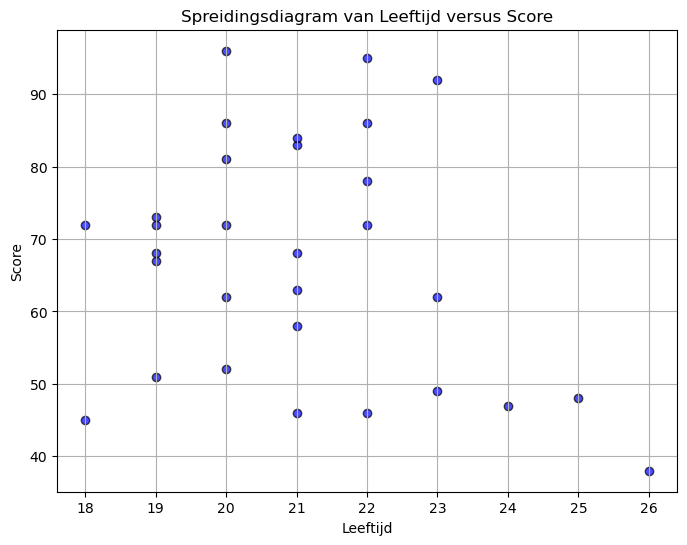
\includegraphics{opg1.7f.png}
            }
        \end{center}
    }
\end{enumerate}

\question{1.15}{Bij een verkeerscontrole zijn de banden van 200 auto's gecontroleerd. Hierbij werd het profiel gemeten in mm.
Een en ander leidde tot de volgende frequentieverdeling (zie de tabel).
    
    \begin{center}
        \begin{tabular}{lc}
            \toprule
            \textbf{Gemeten profiel (in mm)} & \textbf{Aantal auto's} \\
            \midrule
            $0{,}00\,-\,<\,2{,}00$ & 4 \\
            $2{,}00\,-\,<\,4{,}00$ & 34 \\
            $4{,}00\,-\,<\,6{,}00$ & 82 \\
            $6{,}00\,-\,<\,8{,}00$ & 66 \\
            $8{,}00\,-\,<\,10{,}00$ & 14 \\
            \midrule
            \textbf{Totaal} & 200 \\
            \bottomrule
        \end{tabular}
    \end{center}
}

\begin{enumerate}[label=(\alph*)]
    \item Geef de waargenomen verdeling weer door middel van een cumulatieve frequentiecurve.
    \answer{
        De cumulatieve frequentieverdeling is als volgt:
        \begin{center}
            \begin{tabular}{lcc}
                \toprule
                \textbf{Gemeten profiel (in mm)} & \textbf{Cumulatief aantal auto's} \\
                \midrule
                $0{,}00\,-\,<\,2{,}00$ & 4 \\
                $2{,}00\,-\,<\,4{,}00$ & 38 \\
                $4{,}00\,-\,<\,6{,}00$ & 120 \\
                $6{,}00\,-\,<\,8{,}00$ & 186 \\
                $8{,}00\,-\,<\,10{,}00$ & 200 \\
                \midrule
                \textbf{Totaal} & 200 \\
                \bottomrule
            \end{tabular}
        \end{center}

        De cumulatieve frequentiecurve ziet er als volgt uit:

        \begin{center}
            \resizebox{0.9\textwidth}{!}{
                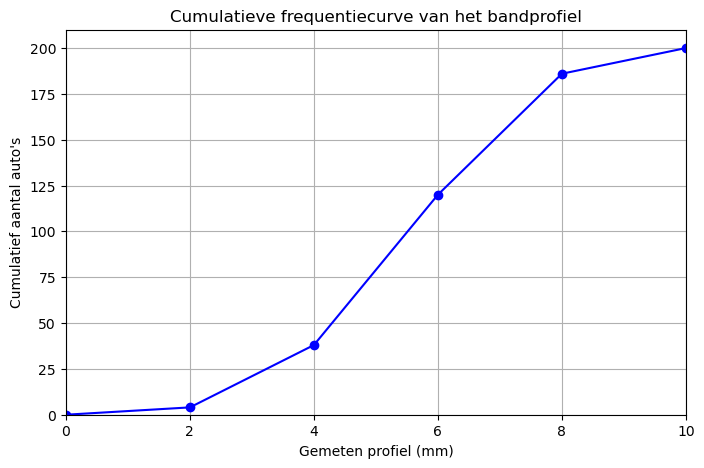
\includegraphics{opg1.15a.png}
            }
        \end{center}
    }
    
    \item Probeer met de grafiek te schatten hoe groot het aantal auto's is met een profiel van minder dan 5,00 mm.
    (NB In deze opgave mag men veronderstellen dat de klassengrenzen exact zijn, dus er hoeven geen correcties met 'halfjes' uitgevoerd te worden.)
    \answer{
        De schatting voor het aantal auto's metg hoogstens een profiel van 5,00mm vinden we
        door te interpoleren op de cumulatieve frequentiecurve van opgave (a).
        Dit ziet er als volgt uit:

        \begin{center}
            \resizebox{0.9\textwidth}{!}{
                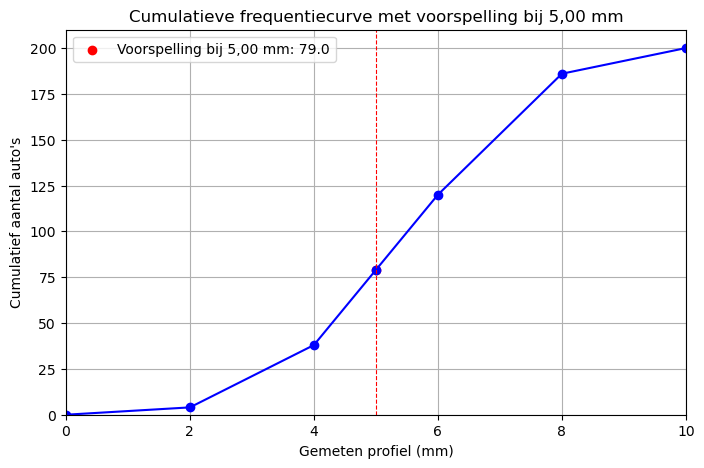
\includegraphics{opg1.15b.png}
            }
        \end{center}

        Naar schatting zullen er dus 79 auto's zijn met een profiel van hoogstens 5,00mm dikte.
    }
\end{enumerate}

\section*{Hoofdstuk 2}
\question{2.m1}{De mediaan van een even aantal waarnemingen is gelijk aan ...}
\begin{enumerate}[label=(\alph*)]
    \item de gemiddelde uitkomst.
    \item de hoogste minus de laagste waarneming gedeeld door twee.
    \item het gemiddelde van de middelste twee waarnemingen na ordening.
    \item het getal dat het meeste blijkt te zijn waargenomen.
\end{enumerate}
\answer{Het juiste antwoord is (c)}

\question{2.m2}{Het gemiddelde maandinkomen van een groep van 15 net-afgestudeerde hbo'ers is 1.850 euro per maand. 
Er blijkt nog een zestiende persoon tot die groep te behoren.
Zijn maandinkomen bedraagt 2.170 euro. 
Van de totale groep van zestien personen is het gemiddelde inkomen dus
}

\begin{enumerate}[label=(\alph*)]
    \item 2.010 euro
    \item 1.870 euro
    \item 2.150 euro
    \item niet te berekenen
\end{enumerate}
\answer{Het juiste antwoord is (b)}

\question{2.m3}{Bij een frequentieverdeling van de gewichten van schapen wordt gewerkt met klassen van 10kg breed.
De gewichten worden op gehele kilogrammen afgerond.
De klasse 20 -< 30 heeft dus als werkelijke bovengrens ...}
\begin{enumerate}[label=(\alph*)]
    \item 10 kg
    \item 29,5 kg
    \item 30 kg
    \item 30,5 kg
\end{enumerate}
\answer{Het juiste antwoord is (b)}

\question{2.m4}{De variantie is ...}
\begin{enumerate}[label=(\alph*)]
    \item slecht hanteerbaar als maatstaf voor spreiding.
    \item de wortel uit de standaarddeviatie.
    \item een grootheid die wordt opgebouwd uit gekwadrateerde afwijkingen van waarneming ten opzicht van het gemiddelde.
    \item het kwadraat van de gemiddelde afwijking.
\end{enumerate}
\answer{Het juiste antwoord is (c)}

\question{2.m5}{Voor een steekproef van 500 werknemers van een groot concern is in 2001 de verdeling van de jaarinkomens onderzocht.
Hierbij bleek dat de standaarddeviatie van de inkomens 7.500 guldens bedroeg.
Ter wille van een internationale publicatie moeten de gegevens worden uitgedrukt in euro's
(1 euro = afgerond 2,20 gulden). De standaarddeviatie gemeten in euro's bedraagt dus ...}
\begin{enumerate}[label=(\alph*)]
    \item 16.500
    \item 36.300
    \item 3.409
    \item 1.100
\end{enumerate}
\answer{Het juiste antwoord is (c)}

\question{2.m6}{In een boxplot kan men diverse kenmerken van een frequentieverdeling aflezen.
Wat kan men hierin echter \emph{niet} aflezen?}
\begin{enumerate}[label=(\alph*)]
    \item de mediaan
    \item het rekenkundig gemiddelde
    \item het eerste kwartiel
    \item de hoogste waarneming
\end{enumerate}
\answer{Het juiste antwoord is (b)}

\question{2.9}{Een groep van 10 studenten behaalde de volgende scores bij een examen:
    \[
        45, 60, 82, 32, 25, 75, 65, 66, 70, 80
    \]
}
\begin{enumerate}[label=(\alph*)]
    \item Bereken het rekenkundig gemiddelde, de mediaan en de standaarddeviatie voor deze gegevens.
    \answer{
        Het rekenkundig gemiddelde wordt berekend met:
        \[
        \samplemean = \frac{\sum x_i}{n} = \frac{45 + 60 + \ldots + 80}{10} = \frac{600}{10} = 60
        \]

        De mediaan wordt gevonden door eerst de scores te sorteren:
        \[
        25, 32, 45, 60, 65, 66, 70, 75, 80, 82
        \]
        Omdat er een even aantal scores is, bekijken we het gemiddelde van de middelste twee waarden:
        \[
        \text{Mediaan} = \frac{x_{5} + x_{6}}{2} = \frac{65 + 66}{2} = 65.5
        \]

        Omdat we te maken hebben met een steekproef, wordt de variantie berekend met:
        \begin{align*}
            \samplevar  &= \frac{1}{n-1}\cdot \sum (x_i - \samplemean)^2 \\
                        &= \frac{1}{10-1} \cdot \left( (45-60)^2 + (60-60)^2 + \ldots + (80-60)^2 \right) \\
                        &= \frac{1}{9} \cdot 3504 \\
                        &= \frac{3504}{9}
        \end{align*}
        De standaarddeviatie vinden we door de wortel uit de variantie te nemen:
        \[
            \samplestd = \sqrt{\samplevar} = \sqrt{\frac{3750}{9}} \approx 19.7315
        \]
    }

    \item Er wordt besloten alle studenten 10 punten extra te geven. Wat is het gevolg van deze maatregel voor de bij vraag (a) berekende maatstaven.
    \answer{
        \textbf{Rekenkundig gemiddelde:} als alle scores met 10 worden verhoogd, dan wordt het rekenkundig gemiddelde ook met 10 verhoogd.

        \textbf{Mediaan:} als alle scores met 10 worden verhoogd, dan geldt dit specifiek ook voor de middelste twee scores (merk op dat de volgorde gelijk blijft!).
        De mediaan is het gemiddelde van de twee middelste scores, dus de mediaan wordt ook verhoogd met 10

        \textbf{Standaarddeviatie}: als alle scores met 10 worden verhoogd, dan blijft de spreiding van de scores gelijk, alleen met 10 naar rechts verschoven.
        De standaarddeviatie blijft in dat geval dus hetzelfde.
    }

    \item In plaats van 10 punten voor iedereen erbij (vraag b) wordt besloten de kandidaten allemaal een 10\% hogere score te geven dan zij oorspronkelijk gehaald hebben. Wat is de invloed van deze maatregel op de onder a berekende grootheden?
    \answer{
        \textbf{Rekenkundig gemiddelde:} als alle scores met 10\% worden verhoogd, dan wordt het rekenkundig gemiddelde ook met 10\% verhoogd.

        \textbf{Mediaan:} als alle scores met 10\% worden verhoogd, dan geldt dit specifiek ook voor de middelste twee scores (merk op dat de volgorde gelijk blijft!).
        De mediaan is het gemiddelde van de twee middelste scores, dus de mediaan wordt ook verhoogd met 10\%

        \textbf{Standaarddeviatie}: als alle scores met 10\% worden verhoogd, dan wordt de spreiding van de scores groter.
        Merk op dat voor elke term $(x_i - \samplemean)^2$ in de formule van de variantie in deze nieuwe situatie moet worden vervangen door 
        \[
            (1.1\cdot x_i - 1.1 \cdot \samplemean)^2 = \left( 1.1 \cdot (x_i-\samplemean)^2\right) = 1.1^2 \cdot (x_i-\samplemean)^2 = 1.21 \cdot (x_i-\samplemean)^2
        \]
        De variantie stijgt dus met een factor $1.21$, en de standaarddeviatie met een factor $\sqrt{1.21}=1.1$ (10\%).
    }
\end{enumerate}      

\question{2.10}{In een gemeente is bijgehouden hoe de prijsontwikkeling is van woningen.
Hierbij wordt een onderscheid gemaakt naar het type woning.
De volgende resultaten zijn verzameld over het afgelopen jaar.
Prijsverandering geeft het verschil aan tussen huidige verkoopprijzen en de prijzen van een jaar geleden.
}

\begin{center}
    \begin{tabular}{cccc}
        \toprule
            \textbf{Type woning} & \textbf{Aantal verkocht} & \textbf{Aantal aanwezig} & \textbf{Prijsverandering} \\
        \midrule
            Villa & $14$ & $280$ & $+5\%$ \\
            Rijtjeshuis & $130$ & $1.600$ & $+2,4\%$ \\
            Appartement & $48$ & $450$ & $+1,6\%$ \\
            Twee onder een kap & $26$ & $500$ & $+7,2\%$ \\
            Serviceflat & $28$ & $140$ & $-2,5\%$ \\
        \bottomrule
    \end{tabular}
\end{center}

\begin{enumerate}[label=(\alph*)]
    \item Bereken voor deze gemeente de gemiddelde prijsverandering van de verkochte huizen.
    \answer{
        De gemiddelde prijsverandering van de verkochte huizen wordt berekend als een gewogen gemiddelde:
        \begin{align*}
            \samplemean &= \frac{14 \cdot 5 + 130 \cdot 2,4 + 48 \cdot 1,6 + 26 \cdot 7,2 + 28 \cdot (-2,5)}{14+130+48+26+28} \\
                        &= \frac{576}{246} \\
                        &\approx 2,3415
        \end{align*}
    }

    \item Bereken op basis van de gegevens de gemiddelde waardeverandering van het totale woningbestand op basis van weging met het aantal aanwezige huizen.
    \answer{
        De gemiddelde waardeverandering van het totale woningbestand wordt berekend als een gewogen gemiddelde:
        \begin{align*}
            \samplemean &= \frac{280 \cdot 5 + 1600 \cdot 2,4 + 450 \cdot 1,6 + 500 \cdot 7,2 + 140 \cdot (-2,5)}{280+1600+450+500+140} \\
                        &= \frac{9210}{2970} \\
                        &\approx 3,1010
        \end{align*}
    }
\end{enumerate}

% \question{2.15}{In een garage heeft men geregistreerd hoelang het uitvoeren van een wintercontrole duurt.
% Van 30 willekeurige auto's in een bepaalde klasse heeft men de tijden in de klassenindeling van bijgaande tabel ondergebracht.
% Bepaal van deze frequentieverdeling achtereenvolgens}

% \begin{center}
%     \begin{tabular}{cc}
%         \toprule
%             \textbf{Tijd (in minuten)} & \textbf{Frequentie} \\
%         \midrule
%             $50-<60$ & $3$ \\
%             $60-<70$ & $8$ \\
%             $70-<80$ & $7$ \\
%             $80-<100$ & $10$ \\
%             $100-<130$ & $2$ \\
%         \bottomrule
%     \end{tabular}
% \end{center}

% \begin{enumerate}[label=(\alph*)]
%     \item de mediaan
%     \answer{

%     }

%     \item de modale klasse
%     \answer{

%     }

%     \item het rekenkundig gemiddelde
%     \answer{

%     }

%     \item de standaarddeviatie
%     \answer{

%     }
% \end{enumerate}

\question{2.20}{Bij een onderzoek in opdracht van Horeca Nederland werd onderzocht hoeveel geld mensen uitgeven aan eten buiten de deur.
Twee groepen werden onderscheiden, namelijk studenten die zelfstandig wonen en afgestudeerden met minstens twee jaar werkervaring.
De resultaten waren als volgt:}

\begin{center}
    \begin{tabular}{c}
        \toprule
            \textbf{Uitgaven voor 30 studenten (euro per maand)} \\
        \midrule
            $72, 51, 146, 30, 28, 88, 92, 47, 52, 68, 80, 34, 28, 105, 76, 93, 55, 40, 62, 37,$ \\
            $88, 30, 122, 46, 35, 29, 77, 40, 71, 57$ \\
        \midrule
            \textbf{Uitgaven voor 40 afgestudeerden (euro per maand)} \\
        \midrule
            $88, 130, 255, 56, 0, 38, 167, 188, 132, 147, 78, 80, 40, 170, 280, 46, 174, 182,$ \\
            $75, 89, 103, 230, 380, 57, 55, 90, 96, 102, 78, 69, 53, 160, 195, 245, 60, 94,$ \\
            $145, 115, 225, 71$ \\
        \bottomrule
    \end{tabular}
\end{center}

\begin{enumerate}[label=(\alph*)]
    \item Bereken voor beide groepen het gemiddelde en de mediaan
    \answer{
        Het gemiddelde wordt berekend als:
        \[
        \samplemean = \frac{\sum x_i}{n}
        \]
        Voor de groep studenten is het gemiddelde gelijk aan:
        \[
        \samplemean_{\text{studenten}} = \frac{72 + 51 + \dots + 57}{30} \approx 62,6333.
        \]
        Voor de groep afgestudeerden is het gemiddelde gelijk aan:
        \[
        \samplemean_{\text{afgestudeerden}} = \frac{88 + 130 + \dots + 71}{40} \approx 125,9500.
        \]

        Aangezien voor beide groepen geldt dat het aantal waarnemingen even is, bekijken we het gemiddelde van de twee middelste waarden.
        Voor de groep studenten is de gesorteerde lijst van waarnemingen gelijk aan:
        \begin{align*}
            &28, 28, 29, 30, 30, 34, 35, 37, 40, 40, 46, 47, 51, 52, 55, 57, 62, 68, 71, 72, 76, 77, 80 \\
            &88, 88, 92, 93, 105, 122, 146
        \end{align*}
        De mediaan is gelijk aan het gemiddelde van de twee middelste waarden, oftewel:
        \[
            \text{Mediaan}_{\text{studenten}} = \frac{55+57}{2} = 56.
        \]
        Voor de groep afgestudeerden is de gesorteerde lijst van waarnemingen gelijk aan:
        \begin{align*}
            &0, 38, 40, 46, 53, 55, 56, 57, 60, 69, 71, 75, 78, 78, 80, 88, 89, 90, 94, 96, 102, \\
            &103, 115, 130, 132, 145, 147, 160, 167, 170, 174, 182, 188, 195, 225, 230, 245, \\
            &255, 280, 380
        \end{align*}
        De mediaan is gelijk aan het gemiddelde van de twee middelste waarden, oftewel:
        \[
            \text{Mediaan}_{\text{afgestudeerden}} = \frac{96+102}{2} = 99.
        \]
    }

    \item Bereken voor beide groepen de standaarddeviatie.
    \answer{
        De variantie wordt berekend als
        \[
            \samplevar = \frac{1}{n-1}\cdot \sum (x_i - \samplemean)^2
        \]
        Voor de groep studenten is de variantie gelijk aan
        \begin{align*}
            \samplevar_{\text{studenten}}   &= \frac{1}{30-1} \cdot \left((72 - 62,6333)^2 + (51-62,6333)^2 + \ldots + (57-62,6333)^2\right)\\                               
                                            &\approx 896,5161.
        \end{align*}
        De standaarddeviatie is de wortel uit de variantie, oftewel
        \[
            s_{\text{studenten}} = \sqrt{\samplevar_{\text{studenten}}} = \sqrt{896,5161} \approx 29,9419.
        \]

        Voor de groep afgestudeerden is de variantie gelijk aan
        \begin{align*}
            \samplevar_{\text{afgestudeerden}}   &= \frac{1}{40-1} \cdot ((88 - 125,9500)^2 + (130-125,9500)^2 + \ldots \\
                                                 & \qquad + (71-125,9500)^2) \\                               
                                                 &\approx 6255,9974.
        \end{align*}
        De standaarddeviatie is de wortel uit de variantie, oftewel
        \[
            s_{\text{afgestudeerden}} = \sqrt{\samplevar_{\text{afgestudeerden}}} = \sqrt{6255,9974} \approx 79,0949.
        \]
    }

    \item Bepaal voor beide groepen een boxplot. Zijn er uitbijters?
    \answer{
        De interkwartielafstand (interquartile range) \( IQR \) wordt berekend als:
        \[
        IQR = Q_3 - Q_1
        \]
        Voor studenten:
        \[
        Q_1 = 37, \quad Q_3 = 80 \Rightarrow IQR_{\text{studenten}} = 43
        \]
        Voor afgestudeerden:
        \[
        Q_1 = 70, \quad Q_3 = 172 \Rightarrow IQR_{\text{afgestudeerden}} = 102
        \]

        Uitbijters worden gedefinieerd als waarden buiten:
        \[
        [Q_1 - 1,5 \times IQR, Q_3 + 1,5 \times IQR]
        \]
        Voor studenten:
        \[
        [37 - 1,5 \times 43, 80 + 1,5 \times 43] = [-27,5, 144,5] \quad \text{Geen uitbijters}
        \]
        Voor afgestudeerden:
        \[
        [70 - 1,5 \times 102, 172 + 1,5 \times 102] = [-83, 325] \quad \text{Uitbijters: 380}
        \]
    }

    \item Schrijf een korte notitie waarin het verschil wordt toegelicht tussen beide groepen.
    \answer{
        Afgestudeerden geven gemiddeld significant meer geld uit aan eten buiten de deur dan studenten. 
        Dit verschil kan worden verklaard door hun hogere inkomen, stabiliteit en veranderde eetgewoonten.
        Daarnaast is de spreiding bij afgestudeerden aanzienlijk groter, wat betekent dat sommige individuen zeer hoge uitgaven hebben.
        De boxplot-analyse bevestigt dat er een uitbijter in de groep van afgestudeerden aanwezig is (380 euro),
        wat mogelijk iemand is met uitzonderlijke uitgavenpatronen.
    }
\end{enumerate}